\section{Zadanie 5}
\subsection{Opis problemu}
Zadanie polegało na znalazieniu wartości zmiennej $ x $, dla której przecinają się wykresy funkcji $ f(x) = 3x $ i $ g(x) = e^{x}$. Wymagana dokładność obliczeń to $ \delta = 10^{-4}$, $\epsilon = 10^{-4}$
\subsection{Rozwiązanie}
W celu wyznaczenia takiego punktu, tj. pary $(x, y)$, zestawiłem ze sobą te funkcje, tj. $ f(x) = g(x) \Rightarrow 3x = e^{x} \Rightarrow 3x - e^{x} = 0$ i przeanalizowalem nowopowstałą funkcję, tj. $ h(x) = 3x - e^{x}$. Za pomocą biblioteki matplotlib wygenerowałem wykres tej funkcji. Z analizy wykresu doszedłem do tego, że funkcja ta ma dwa miejsca zerowe, jedno wśród argumentów z zakresu $ x \in  (0.0, 1.0) $ oraz drugie z zakresu $ x \in (1.0, 2.0) $. W związku z zaobserowanymi własnościami funkcji $ h(x) $ za pomocą funkcji $ \texttt{mbisekcji} $ odnalazłem miejsca zerowe z dokładnością wymaganą w treści zadania.

\begin{figure}[!htbp]
  \centering  
  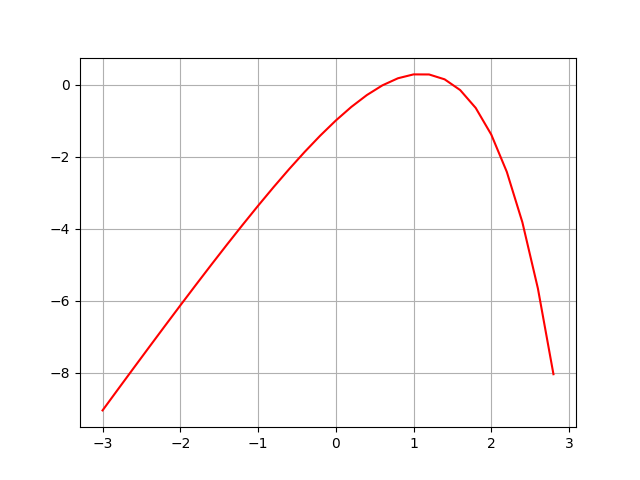
\includegraphics[totalheight=6cm]{../plots/ex5.png}
  \caption{Wykres $g(x) = 3x - e^{x}$}
\end{figure}

\subsection{Wynik}
Wyniki zestawiłem w tabeli poniżej: \\
\begin{center}
\begin{tabular}{|c|c|c|c|c|}
  \hline 
    Przedział & $x$ & $ f(x)$ & $i$ & $err$ \\
  \hline
  $ (0.0, 1.0) $ & 0.619140625 & 9.066320343276146e-5 & 9 & 0\\
  \hline 
  $ (0.1, 2.0) $ & 1.5120849609375 & 7.618578602741621e-5 & 13 & 0\\
  \hline
\end{tabular} 
\end{center}

\ \\
Porównując (w pakiecie matematycznym) wyniki uzyskane za pomocą metody bisekcji z rzeczywistymi wartościami, możemy stwierdzić, że wartości te są poprawne (z uwzględnieniem błędu). W metodzie bisekcji bardzo ważnym jest, aby odpowiednio dobrać przedziały (warunki początkowe). Próby eksperymentalnego znalezienia miejsc zerowych na przedziale $ \langle0, 2\rangle $ nie doprowadziły do poprawnego wyniku. (nie spełniał on założenia o różnych znakach wartości na krańcach przedziału)